\documentclass[12pt, a4paper]{article}
\usepackage{geometry}
\usepackage{booktabs}
\usepackage{diagbox}
\usepackage{graphicx}
\usepackage{ragged2e}
\usepackage{tabularx}
\usepackage{fancyhdr}
\usepackage{palatino}
\usepackage{tikz}
\usepackage{amsthm}
\usepackage{leftidx}
\usetikzlibrary{shapes.geometric, arrows}

\parindent 0pt
\parskip 5pt
\pagestyle{fancy}

\fancyhead[L]{Consensus}
\fancyhead[R]{COMP90020 Distributed Algorithms}
\fancyfoot[L]{Semester 1, 2020}
\fancyfoot[C]{}
\fancyfoot[R]{\thepage}
\fancypagestyle{firststyle}{%
  \fancyhf{}
  \fancyfoot[L]{Semester 1, 2020}
  \fancyfoot[R]{\thepage}
  \renewcommand{\headrulewidth}{0pt}
}
\renewcommand{\headrulewidth}{0.4pt}
\renewcommand{\footrulewidth}{0.4pt}

\title{\textsc{Consensus}}
\author{
  Qifan Deng \\
  \texttt{\small qifand@student.unimelb.edu.au}
  \and
  Zhaofeng Qiu \\
  \texttt{\small zhaofengq@student.unimelb.edu.au}
  \and
  Alan Ung \\
  \texttt{\small alanu@student.unimelb.edu.au}
  \and
  Yangzhe Xie \\
  \texttt{\small yangzhex@student.unimelb.edu.au}
  \and
  Min Zhao \\
  \texttt{\small zhaomz1@student.unimelb.edu.au}
}
\date{Semester 1, 2020}

\newtheorem*{assumption*}{\assumptionnumber}
\providecommand{\assumptionnumber}{}
\makeatletter
\newenvironment{assumption}[2]
 {
  \renewcommand{\assumptionnumber}{Assumption #1}
  \begin{assumption*}%
  \protected@edef\@currentlabel{#1}
 }
 {
  \end{assumption*}
 }
\makeatother
\newcommand{\asref}[2]{\ref{#1}}

\begin{document}
\maketitle
\thispagestyle{firststyle}


\section{Introduction}

Achieving agreement among remote processes in a distributed system is a
fundamental problem relevant to a wide range of applications
\cite{fischer1985impossibility, kshemkalyani_singhal_2008}. Indeed, many common
tasks---such as coordinating access to shared resources, electing a leader and
achieving agreement on message delivery order---share the core requirement for
processes to communicate and negotiate with each other to establish a common
understanding before taking further action \cite{kshemkalyani_singhal_2008,
coulouris2005distributed}.

The \textit{consensus} problem generalises these tasks to ask how a collection
of processes can agree on a value $v$, no matter the domain from which $v$ may
be taken \cite{coulouris2005distributed}. Due to issues such as node failures
and network unreliability, it can be difficult to achieve consistency among
nodes in distributed computing or multi-agent systems
\cite{coulouris2005distributed}. Therefore, the algorithms used to achieve
consensus must take failures into consideration and aim to be as robust as
possible.

This report first provides a formal definition of the consensus problem in
\S\ref{sec:consensus-def}, alongside a brief introduction to two closely related
problems. We then introduce the \textit{CAP} theorem in \S\ref{sec:cap-theorem},
outlining a key limitation of distributed systems before discussing important
fundamental models in \S\ref{sec:fundamental-models} which are important to
consider when comparing and analysing different distributed algorithms. In doing
so, we will discover that under a certain fundamental model, no algorithm can
guarantee consensus under all circumstances.

To further motivate the consensus problem and expand on its aforementioned
fundamentality to many applications, we discuss in detail a range of relevant
tasks in \S\ref{sec:relevant-problems}. We then focus on two algorithms by which
to achieve consensus. \textit{Paxos} \cite{lamport1998part, lamport2001paxos}
(detailed in \S\ref{sec:paxos}) has been the dominant consensus algorithm for
much of the past two decades, underpinning most implementations of consensus
\cite{ongaro2014search}. More recently, however, a contending consensus
algorithm has been proposed. Raft \cite{ongaro2014search} (detailed in
\S\ref{sec:raft}) is purported by its authors to ``[produce] a result equivalent
to (multi-)Paxos'' and be ``as efficient as Paxos'' yet ``more understandable''
and able to ``provide a better foundation for building practical systems.''
\cite{ongaro2014search} We provide a detailed comparative analysis between the
two in \S\ref{sec:analysis}, discussing the benefits and drawbacks of either
algorithm. Finally, we discuss our own implementation of the
\textbf{(Paxos/Raft)} algorithm as part of a \textbf{(application type)}
application, providing a case study of the algorithm in a concrete context.


\section{Formal Definition}

\subsection{Consensus Problem} \label{sec:consensus-def}

The consensus problem is defined with respect to a collection of $N$ processes
which communicate by message passing. Every process $p_{i}$ $(i = 1, \ldots, N)$
begins in the \textit{undecided} state, in which they each propose a single
value $v_{i} \in D$, where $D$ is a set of acceptable values
\cite{coulouris2005distributed}.

The processes then exchange values with each other. During this phase, each
process sets the value of its \textit{decision variable}, $d_i$ $(i = 1, \ldots,
N)$, based on the information obtained from other processes. In doing so, they
enter the \textit{decided} state, in which the decision variable may no longer
change.

A consensus algorithm must satisfy the following conditions for every execution:

\begin{itemize}
  \item \textbf{Termination}: Each non-faulty process $p_i$ must eventually set
    $d_i$.
  \item \textbf{Agreement}: All non-faulty processes in the decided state
    must have the same value. If $p_{i}$ and $p_{j}$ are correct and have
    entered the decided state, then $d_{i} = d_{j}$ $(i, j = 1, \ldots, N)$.
  \item \textbf{Integrity/Validity}: If all non-faulty processes proposed
    the same value, then the decision variable of all non-faulty processes is
    that same value.
\end{itemize}

There are two other problems similar to the consensus problem---the
\textit{Byzantine generals problem} (also known as the \textit{Byzantine
agreement problem}) and the \textit{interactive consistency problem}. Table
\ref{tab:dbtap} provides a comparison between these and the consensus problem.
Despite the differences in requirements, a solution to any one of them can be
transformed to one of the others by reduction \cite{fischer1983consensus}.

\begin{table}[htp]
  \centering
  \begin{tabularx}{\linewidth}{%
    l%
    >{\raggedright\arraybackslash}X%
    >{\raggedright\arraybackslash}X%
    >{\raggedright\arraybackslash}X}
  \toprule
  Condition & Consensus & Byzantine Generals & Interactive Consistency \\
  \midrule
  \textbf{Termination} & Eventually decide on a \textit{value}
    & Eventually decide on a \textit{value}
    & Eventually decide on an \textit{array $A$} \\
  \addlinespace
  \textbf{Agreement} & Agree on the same value
    & Agree on the same value
    & Agree on the same array of values $A[v_{1} \ldots v_{n}]$ \\
  \addlinespace
  \textbf{Integrity}
    & The decided value is based on the propositions of all correct processes
    & If the commander is correct, then all correct processes decide on the
      value proposed by it
    & All correct processes decide on $v_{i}$ as the $i\textsuperscript{th}$
      component of their vector if $p_{i}$ is correct \\
  \bottomrule
\end{tabularx}
  \caption{Comparison of similar problems}
  \label{tab:dbtap}
\end{table}

\subsection{CAP Theorem} \label{sec:cap-theorem}

The CAP theorem \cite{brewer2012cap} states that, in a distributed system, it is
impossible for an algorithm to provide more than two of these three properties:

\begin{itemize}
	\item \textbf{Consistency}: All data backups in the distributed system have
    the same value at the same time.
	\item \textbf{Availability}: After some nodes in the cluster fail, the entire
    cluster can still respond to client read and write requests. However, there
    is no guarantee that the data produced is most up-to-date.
	\item \textbf{Partition tolerance}: The system continues to operate despite
    delayed, lost or dropped messages on the network.
\end{itemize}

%% Maybe include in the future.
% \subsection{ACID Theorem}

\subsection{Models of Computation} \label{sec:fundamental-models}

Solving the consensus problem varies in difficulty depending on the system model
being considered. Different models assert different assumptions and thus, it is
important to consider the impacts of such models on the consensus algorithms to
be investigated.

\subsubsection{Synchronous and Asynchronous Systems}

\textit{Fundamental models} provide an ``abstract perspective'' for considering
individual aspects of a distributed system \cite{coulouris2005distributed}. An
\textit{interaction model} is a fundamental model concerned with communication
and coordination between processes, including aspects such as process execution,
message delivery and clock drift \cite{coulouris2005distributed}. Although it is
difficult to set limits on these, considering ``two extremes of a spectrum''
gives rise to a pair of simple models---one with strong assumptions about time
and the other with none \cite{coulouris2005distributed, hadzilacos1994modular}.

The \textit{synchronous} system model is defined by Hadzilacos and Toueg
\cite{hadzilacos1994modular} to be one in which:

\begin{enumerate}
  \item Time taken by a process to execute a step has known upper and lower
    bounds.
  \item Every process has a local clock whose drift rate has a known bound.
  \item There is a known upper bound on message delay.
\end{enumerate}

These bounds are global across the entire system. A collection of processors
connected by a communication bus is an example of a system which closely aligns
to the synchronous model.

By contrast, the \textit{asynchronous} system model is one which makes no
assumptions about time \cite{coulouris2005distributed, hadzilacos1994modular}.
Namely, there are no bounds on process execution time or message transmission
delay and clock drift rates may be arbitrarily fast or slow
\cite{coulouris2005distributed}. This model is useful when considering systems
such as the Internet \cite{coulouris2005distributed}.

The asynchronous model is more general than the synchronous counterpart. As
such, it is more difficult to solve the consensus problem under the former than
the latter. An algorithm which works under the asynchronous model will also work
for the synchronous model.

The consensus problem is solvable under the synchronous model
\cite{fischer1985impossibility, kshemkalyani_singhal_2008}. However, it has been
shown by Fischer \cite{fischer1985impossibility} to be impossible to solve under
the asynchronous model. No matter the protocol or algorithm, there is always a
``window of vulnerability'' during which the failure of processes or delay of
messages prevents the system from reaching consensus by way of nontermination
\cite{fischer1985impossibility}. Despite this, it should be noted that the
impossibility arises from a worst-case scenario of low probability---in reality,
process scheduling has aspects of randomness \cite{aguilera2010stumbling}. Thus,
although it is not theoretically possible to guarantee consensus under the
asynchronous model in all circumstances, consensus algorithms can still be
implemented in practice.

\subsubsection{Byzantine and Crash Failures}

A consensus algorithm may be classified as either of the following, depending on
the types of failures it can handle.

\begin{itemize}
	\item Byzantine Fault Tolerant (BFT): if the algorithm can handle arbitrary
    faults, including those arising from malicious actions of an adversary.
	\item Crash Fault Tolerant (CFT): if the algorithm can handle failures caused
    by process crashes or fail-stops.
\end{itemize}

Any BFT algorithm is also a CFT algorithm, since Byzantine failures encompass
all possible faults in the system model. The hierarchy of different faults
\cite{barborak1993consensus} is shown in Figure \ref{fig:aofc}.

\begin{figure}[htp]
  \centering
  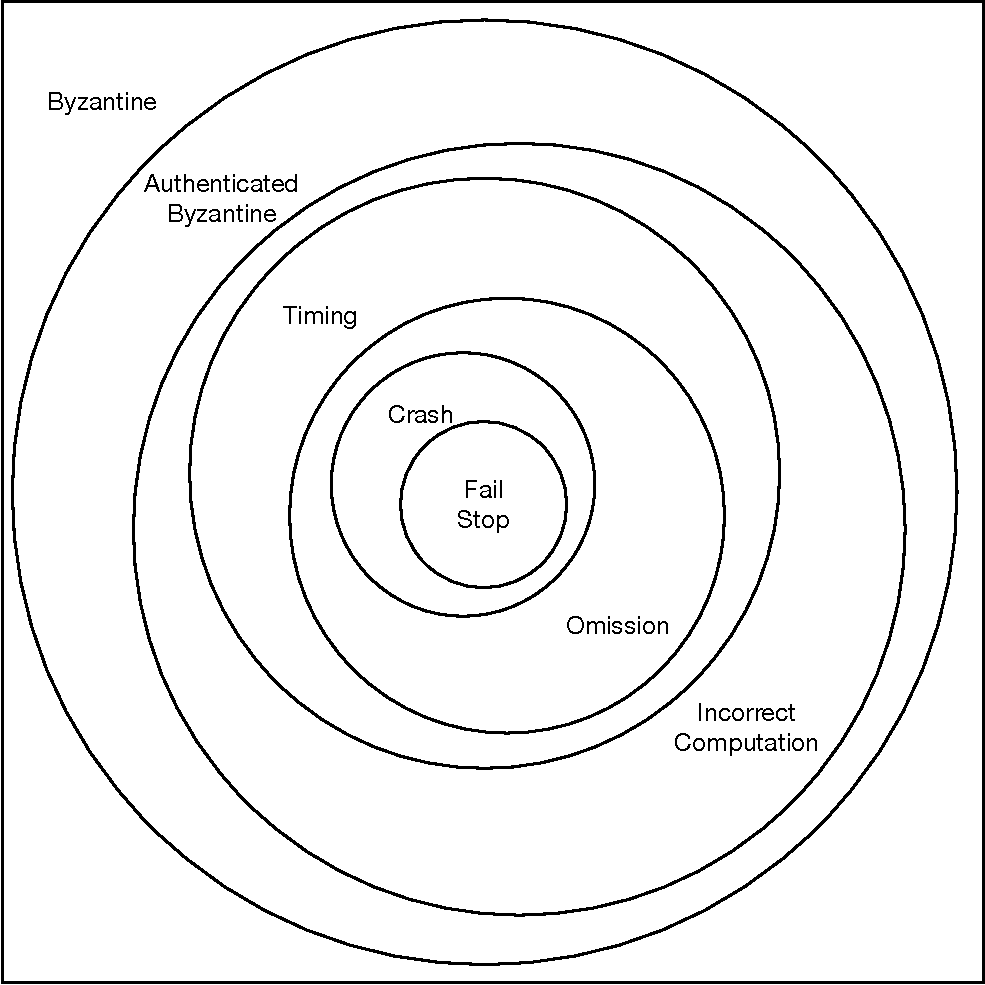
\includegraphics[width=0.8\textwidth]{img/AOFC.pdf}
  \caption{An ordered fault classification (Barborak et al.)}
  \label{fig:aofc}
\end{figure}


\section{Relevant Problems} \label{sec:relevant-problems}

The consensus problem lies at the core of many problems in distributed
computing, making effective solutions to it highly desirable
\cite{fischer1985impossibility}. To motivate consensus in context, related
problems---highlighting useful applications in distributed computing---are
discussed in this section.

\subsection{Reliable Multicast}

Ensuring that all processes receive updates in the same order.

\subsection{Membership/Failure Detection}

Ensuring that every process has a local record containing every other process.
Failures should be detected and records should be updated.

\subsection{Leader Election}

Deciding on a leader among all processes, with all processes being aware of
who the leader is.

\subsection{Mutual Exclusion}

Ensuring that simultaneous access to a resource does not occur (exclusive
access).


\section{Paxos Algorithm} \label{sec:paxos}

Draft: What Paxos do we have?

Paxos \cite{lamport2001paxos}, Fast Paxos \cite{fastpaxos}, 
S-Paxos \cite{spaxos}, 
OpenReplica \cite{openreplica} and Ring Paxos \cite{ringpaxos}.

\begin{figure}[htp]
  \centering
  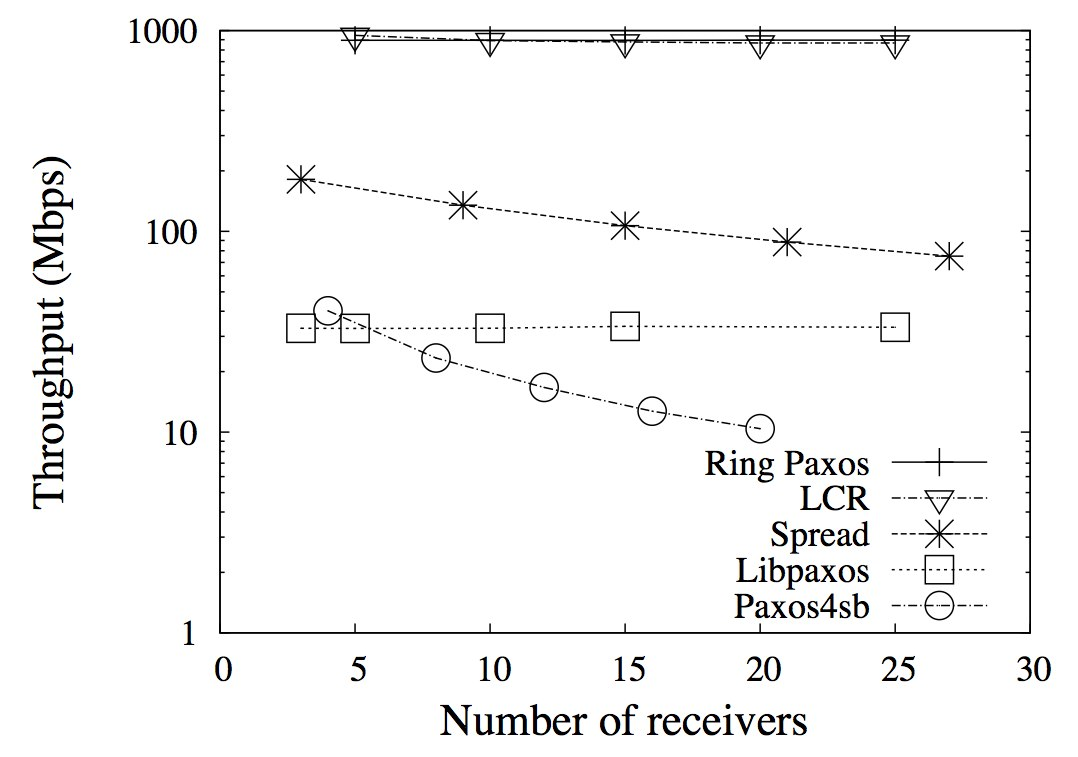
\includegraphics[width=0.8\textwidth]{img/RingPaxosThroughput.jpg}
  \caption{Ring Paxos Throughput}
  \label{fig:RingPaxosThroughput}
\end{figure}


\subsection{Problem}
In distributed computing, there are processes cooperating with each other. 
Paxos is designed to achieve consensus which ensures 
only a single value is chosen from proposed values that 
proposed by some processes\cite{fischer1983consensus}. 
After been chosen, this value is also available to be learnt by all processes
when a process can only learn a value that has beed chosen.

\paragraph{}
The following content of this section explains 
Paxos algorithm based on \cite{fischer1983consensus}. 
In their work, they make two assumptions, 
based on that, they then give principles to solve the consensus problem. 
These principles require a proposing approach 
of which each proposal has an ordered number \textit{n} 
and a proposal value \textit{v}. 
The principles also require three classes of agents 
which are proposers, acceptors and learners. 
There are two phases when choosing a value.
\textit{Phase1} is to \textit{prepare} a proposal 
by requesting a majority of acceptors. 
\textit{Phase2} is to ask the majority to \textit{accept} this proposal.
In this phase, any acceptor among the majority can 
either accept or decline the \textit{accept} request.

\subsection{Two Assumptions}
\begin{quote}
  \begin{assumption}{1}{F}\label{as:1}
    Processes run asynchronously. 
    They may have arbitrary running speed, may fail and may restart.
  \end{assumption}
  \begin{assumption}{2}{F}\label{as:2}
    Processes can communicate with each other by message passing. 
    Messages can take arbitrarily long to be delivered. 
    Messages can be duplicated, can be lost, but can not be corrupted.
  \end{assumption}
\end{quote}
\subsection{Two Principles}

The principles are given here and will be applied later,
\begin{quote}
  P1. An acceptor must accept the first proposal that it receives.
  \begin{quote}
    a. An acceptor can accept a proposal numbered \textit{n} 
      iff it has not responded to a \textit{prepare} request 
      having a number greater than \textit{n}.
  \end{quote}
  P2. If a proposal with value \textit{v} is chosen, 
    then every higher-numbered proposal that is chosen has value \textit{v}
    \begin{quote}
      a. If a proposal with value \textit{v} is chosen, 
        then every higher-numbered proposal accepted 
        by any acceptor has value \textit{v}.
        
      b. If a proposal with value \textit{v} is chosen, 
        then every higher-numbered proposal issued 
        by any proposer has value \textit{v}.

      c. For any \textit{v} and \textit{n}, 
        if a proposal with value \textit{v} 
        and number \textit{n} is issued,
        then there is a set \textit{S} consisting of 
        a majority of acceptors such that either 
          \begin{quote}
            (i) no acceptor in \textit{S} has accepted 
              any proposal numbered less than n, or 
              
            (ii) \textit{v} is the value of 
              the highest-numbered proposal among 
              all proposals numbered less than 
              \textit{n} accepted by the acceptors in \textit{S}.
          \end{quote}
  \end{quote}
\end{quote}

\subsection{Three Agents}

To achieve the consensus, there are three classes of agents 
which are proposers, acceptors and learners. 
When a process proposes a proposal, 
it is included in the class of proposers.
When a process receive requests from any of the proposers,
it is then included in the class of acceptors.
And when a process learn a chosen value, 
it is included in the class of learners.
These three cases can happen simultaneously, i.e.
a process can propose, receive requests or 
learn a chosen value at the same time.
Thus the three classes of agents are 
not mutually exclusive for a single process.


\subsection{Implementation}
\subsubsection{Choosing A Value}\label{Choosing}
The Paxos algorithm \cite{lamport1998part} chooses a leader 
from the processes of assumption \ref{as:2}. 
This leader is the leader of the class of proposers and 
also the leader of the class of learners at the same time. 
A proposal is tagged with an ordered number \textit{n} and a value \textit{v}.
The proposal will be passed from one proposer to the leader. 
This leader is in charge of requesting a majority of accepters to ask for 
acceptance.
The majority can be generated by the algorithm \cite{keidar2001cost}.
A proposal will be requested two times to finally be chosen.
At the first time request, named \textit{prepare} request, 
an acceptor should respond the proposer leader with a \textit{promise} respond.
Once get \textit{promise} respond from a majority 
(this majority could be different from the requested one),
the proposer leader requests each \textit{promised} acceptor 
in the majority with an \textit{accept} request 
to confirm the acceptance of this proposal.
The acceptor which receives this \textit{accept} request 
will accept this proposal based on $P1^a$. 
And no matter it accepts it or not, it should respond the proposer leader to
confirm their reaction.
If a proposal was proposed, i.e. a value was chosen, 
then it comes to learn it.

\subsubsection{Learning A Value}
There are three easy approaches to learn a value.
The first, in \textit{Phase2}, when acceptors accept a value, 
they can respond to all the learners. 
This is immediate but requires a response number at
the product of the number of learners and the number of acceptors.
The second, accepters now respond only the leader of learners. 
However, this is unreliable since we have the assumption\ref{as:2}.
It brings us to the third way, which is to have a set of leaders of learners
combining the benefits of the other approaches without lots of message passing.
\paragraph{}
The three ways above are all passive in the perspective of a learner when
it is actually be notified what the chosen value is.
If a learner want a chosen value itself, 
it can get an another agent to be  a proposer 
to propose a proposal using the above algorithm. 
\subsection{Protocol}
\cite{PaxosMadeSwitch-y} uses UDP to pass messages, 
they think Paxos does not require reliable communications, 
so using TCP is unnecessary.
\subsection{Issues}
Because of assumption\ref{as:1} and 
the use of a quorum of acceptors \cite{jalili2014practical}, 
with that acceptors handling messages sequentially,
performance hiccups may occurs when it takes time for slower acceptors 
to catch up.
\subsubsection{Contention}

\subsection{Optimisations}
To prevent failures described in assumption\ref{as:1}, 
stable storage is used by both proposers and acceptors.
The highest-numbered proposal is always stored in a proposer's stable storage.
The intended response is always stored in an acceptor's stable storage
before it responds.

\section{Raft algorithm} \label{sec:raft}
The Raft algorithm was proposed in 2014\cite{conf/usenix/OngaroO14} as an alternative to the (Multi-)Paxos algorithm, which is more
understandable and easier to implement a practical system. The highlight of the Raft algorithm is that it adopts an
engineering thinking --- It simplifies the model of the design according to the requirements in practical applications and
modularizes the process of the algorithm. From the perspective of performance and security, the Raft algorithm is also almost
the same as Paxos.
\subsection{Roles}
  \subsubsection{Follower}
  All nodes are followers when they are started. The followers are completely passive, they can only respond to the incoming
  messages. If the client's message is sent to a follower, the message will be redirected to the leader of this cluster. Followers may
  also be able to become a leader through elections under certain conditions.
  \subsubsection{Leader}
  There can be only one Leader in the entire cluster at the same time. The leader handles all client interactions.
  \subsubsection{Candidate}
  The candidate state is a state between the follower state and the leader state. When a follower becomes a candidate, an election
  will be held. The candidate who wins the election will be the new leader.
\subsection{Protocol}
In the Raft algorithm, time is divided into terms, Each term has a number, and the number increments when a new term starts. Each term starts
with an election. If the election is successful, then the chosen leader will serve out for the rest of the term, which means that
only one leader can be elected in a given term. If the election is not successful, then the candidate starts a new term. Each node
in the cluster maintains the value of the current term number and it should be stored reliably. The function of the term and term number is
to allow the nodes to identify the information that is out of date.
\par
In order to let the followers believe there is an active leader in the cluster, followers expect to receive heartbeat messages from
the leader regularly. If the follower's timeout of heartbeat message elapses, it assumes that the leader crashed and will start a
new election. This timeout is often much longer than the propagation time of the message in the network.
\par
There are only two type of RPCs in the Raft algorithm:
\begin{itemize}
  \item \textbf{RequestVote RPC}: invoked by candidates to gather votes from other nodes.
  \item \textbf{AppendEntries RPC}: invoked by the leader to replicate log entries.
\end{itemize}
  \subsubsection{Leader Election}
  When a node begins an election, the first thing it does is to increment its current term number. The node then converts itself from
  follower state to candidate state. To win the election, the node must receive votes from a majority of nodes in the cluster. The node
  votes for itself, then send RequestVote RPCs to all other nodes and retry this process until:
  \begin{itemize}
    \item It receives votes from majority of nodes in the cluster, which means it wins the election and becomes the leader.
    \item It receives a RPC from a leader, which means one of other candidates wins the election, the current node becomes a follower.
    \item Election timeout elapses, which means no one wins the election. The node will then increment the term number and start a new election
  \end{itemize}
  \par
  To ensure safety, each node can only give out at most one vote in a term. This guarantees that only one candidate can get votes from
  the majority in the same term, thus only one candidate can win the election. Also, to prevent live lock of the election, the election
  timeout of each node is chosen randomly.
  \subsubsection{Log Replication}
  Once a leader is elected, it receives all client's request messages. These messages contain a command to be executed by the replicated
  state machine. The leader creates a log entry for each request from the clients. Apart from commands, the log entry also contains an index
  number in the log and a term number when the log entry was first created. Each log entry is committed if known to be stored in the logs of
  the majority of the nodes.
  \par
  When the leader receives a command from a client, it appends the command with the current term number and index number to its log. Then the leader
  sends AppendEntries RPCs to all followers. Once a new log entry is committed, the leader passes the command to its state machine and
  notifies all followers of this new log entry. When the followers receive these RPCs, they pass the command to their state machine.
  \par
  To ensure consistency of logs, each AppendEntries RPC contains the index and the term of the previous log entry. The followers who receives the RPC will
  reject the request if they do not have a matching log entry. It then is guaranteed that a new entry is only accepted if the logs match in
  their previous entry. So if a given log entry is committed, its all previous log entries are also committed.
  \par
  At the beginning of a new leader's term, the old leaders may have left some log entries that are partially replicated. The way that the Raft
  algorithm used to solve this problem is to force all follower to duplicate its log, which will also force all follower to discard all the
  inconsistent log entries and fill in all missing log entries. The leader maintains a value nextIndex for each follower, which marks the index
  of the next log entry to send to that follower. When AppendEntries consistency check fails, it decrements the nextIndex and retries until the
  follower's log is repaired.
  \subsubsection{Safety}
  If a leader has decided that a log entry is committed, then that entry should be present in the logs of all future leaders. To guarantee this,
  the algorithm picks the candidate to win the election such that it has the log that is most likely to have all the entries that have been
  committed. So the candidates must include log info in RequestVote RPCs including index and term of the last log entry. And the voting servers
  have to deny if its log is more complete.
  \par
  Another safety issue is that if a leader crashes while replicating logs, the new leader will not know whether the last log entry of the
  previous leader has been committed or not. To solve this problem, a new commitment rule must apply --- For a leader to decide an entry
  is committed, in addition to the previous rule, at least one new entry from leader's term must also be stored on the majority of servers.
\subsection{Issues}

\subsection{Optimisations}


\section{Comparative analysis} \label{sec:analysis}


\section{Application} \label{sec:application}


\bibliographystyle{ieeetr}
\bibliography{main}

\end{document}
